\chapter{Implementasi dan Pengujian}
\label{chap:implementasidanpengujian}

Bab ini membahas mengenai implementasi dan pengujian perangkat lunak SharIF Judge.

\section{Lingkungan Implementasi dan Pengujian}
\label{sec:5:lingkungan}

Implementasi perangkat lunak dilakukan pada beberapa lingkungan yang berbeda:

\begin{itemize}
    \item Lingkungan \textit{development}: \\ Perangkat lokal milik penulis yang digunakan untuk pembangunan perangkat lunak. Spesifikasi lingkungan ini adalah sebagai berikut:
    \begin{itemize}
        \item Perangkat Keras:
        \begin{itemize}
            \item \textit{Processor}: Intel Core i5-7600 3.5GHz
            \item \textit{Random Access Memory}: 16GB DDR4
            \item \textit{Storage}: 500GB
        \end{itemize}
            \item Perangkat Lunak:
        \begin{itemize}
            \item \textit{Operating System}: Windows 10 Home 64-bit
            \item \textit{Windows Subsystem for Linux}: Ubuntu 20.04.2 LTS
        \end{itemize}
    \end{itemize}
    
    \item Lingkungan \textit{staging}: \\ Lingkungan \textit{server} yang digunakan untuk menguji perangkat lunak selama pembangunan. Spesifikasi lingkungan ini adalah sebagai berikut:
    \begin{itemize}
    \item Perangkat Keras:
        \begin{itemize}
            \item \textit{Processor}: Intel DO-Regular 2.4GHz
            \item \textit{Random Access Memory}: 1GB
            \item \textit{Storage}: 25GB
        \end{itemize}
            \item Perangkat Lunak:
        \begin{itemize}
            \item \textit{Operating System}: Ubuntu 20.04.3 LTS
        \end{itemize}
    \end{itemize}
    
    \item Lingkungan \textit{production}: \\ Lingkungan \textit{server} yang digunakan pada kuliah Dasar-dasar Pemrograman dengan alamat \verb|http://daspro.labftis.net|. Spesifikasi lingkungan ini adalah sebagai berikut:
    \begin{itemize}
    \item Perangkat Keras:
        \begin{itemize}
            \item \textit{Processor}: Intel Xeon E5-2603 1.70GHz
            \item \textit{Random Access Memory}: 8GB
            \item \textit{Storage}: 1TB
        \end{itemize}
            \item Perangkat Lunak:
        \begin{itemize}
            \item \textit{Operating System}: Ubuntu 16.04.6 LTS
        \end{itemize}
    \end{itemize}
\end{itemize}

\section{Implementasi}
\label{sec:5:implementasi}

\subsection{Tampilan Antarmuka}
\label{subsec:5:antarmuka}

\begin{figure}[H]
	\centering  
	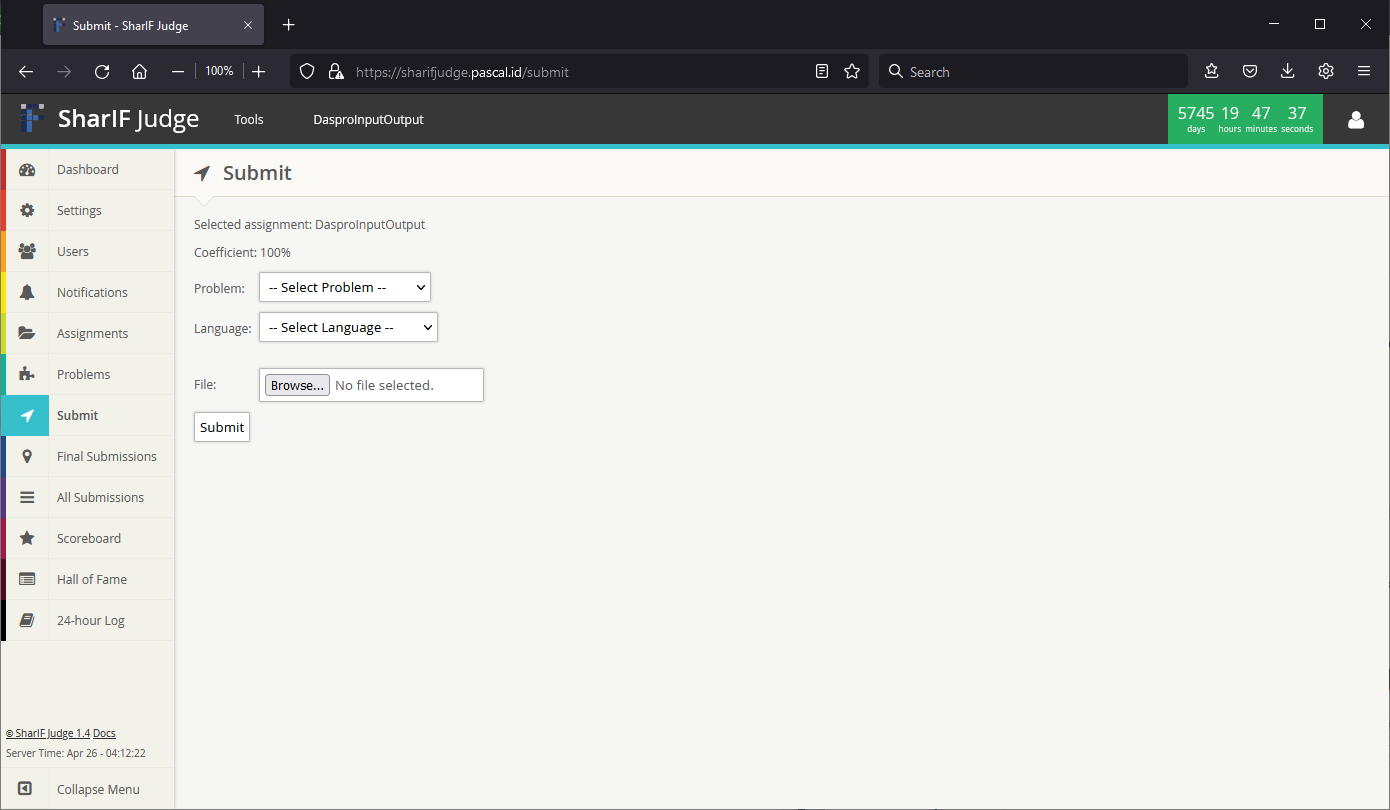
\includegraphics[scale=0.4]{submit}  
	\caption{Tampilan antarmuka halaman Submit} 
	\label{fig:5:antarmuka} 
\end{figure}

Gambar \ref{fig:5:antarmuka} merupakan tampilan antarmuka pada halaman Submit yang sudah diimplementasikan. Seluruh perubahan pada \verb|submit.twig| terdapat pada lampiran \ref{lampA:Submit.twig}. Seluruh \textit{style} dan \textit{script} untuk halaman ini terletak di \textit{file} terpisah. \textit{Stylesheet} yang terdapat di \verb|assets\styles\submit.css| terdapat pada lampiran \ref{lampA:submit.css}. \textit{Script} yang terdapat di \verb|assets\js\shj_submit.js| terdapat pada lampiran \ref{lampA:shj_submit.js}.

\subsection{Menampilkan Soal}
\label{subsec:5:soal}

Soal PDF ditampilkan pada \verb|iframe| yang berisi \verb|viewer.html| milik PDF.js. URL dari \textit{file} PDF yang akan ditampilkan adalah URL yang mengarah ke fungsi \verb|pdf| pada controller \verb|Assignments|. URL ini dikirim ke \verb|viewer.html| milik PDF.js sebagai parameter GET bernama \verb|site_url|.

Fungsi \verb|pdf| pada controller \verb|Assignments| menggunakan fungsi \verb|force_download| yang menyebabkan munculnya dialog unduh pada \textit{browser}. Agar \textit{file} PDF dapat dibaca oleh \textit{browser} dan tidak memunculkan dialog unduh, \textit{file} PDF akan dikembalikan dengan fungsi \verb|echo| dengan header \verb|Content-Type: application/pdf|. Ditambahkan parameter \verb|$no_download| pada fungsi \verb|pdf| untuk menentukan apakah \textit{file} PDF soal akan diunduh atau ditampilkan oleh PDF.js. Jika \verb|$no_download| bernilai \verb|FALSE|, maka PDF akan diunduh melalui fungsi \verb|force_download| seperti semula. Jika \verb|$no_download| bernilai \verb|TRUE|, maka isi PDF akan dikembalikan melalui fungsi \verb|echo| dengan \textit{header} \verb|Content-Type: application/pdf|. Kode untuk perubahan ini terdapat pada lampiran \ref{lampA:Assignments.php}

\subsection{Editor Kode}
\label{subsec:5:editor}

Ace menggunakan sebuah elemen \verb|div| sebagai tempat untuk menampilkan editor kodenya. Editor Ace dimuat dan dikonfigurasi melalui JavaScript yang terdapat di \verb|shj_submit.js|. Ditambahkan juga beberapa fungsi untuk mengubah konfigurasi \textit{syntax highlighting} sesuai dengan bahasa yang dipilih, dan untuk mengaktifkan atau menonaktifkan editor kode jika \textit{problem} dan bahasa belum dipilih. Kode JavaScript untuk konfigurasi editor Ace terdapat pada lampiran \ref{lampA:shj_submit.js}.

\subsection{Menyimpan dan Memuat Kode}
\label{subsec:5:simpan}

Kode akan disimpan pada \textit{file} txt bernama \verb|editor.txt|. Nama dan tipe file ini disimpan sebagai konstanta pada \verb|constants.php|. Perubahan kode \verb|constants.php| terdapat pada lampiran \ref{lampA:constants.php}.

Untuk menyimpan kode, fungsi \verb|save| ditambahkan pada \textit{controller} \verb|Submit|. Fungsi ini mengambil isi dari editor kode melalui POST lalu menyimpannya pada \verb|editor.txt|. Kode untuk fungsi \verb|save| terdapat pada lampiran \ref{lampA:Submit.php} baris 72--135.

Untuk memuat kode, fungsi \verb|load| ditambahkan pada \textit{controller} \verb|Submit|. Bila tersedia, fungsi ini mengambil isi dari \verb|editor.txt| txt lalu mengembalikan isinya. Kode untuk fungsi \verb|load| terdapat pada lampiran \ref{lampA:Submit.php} baris 39--64.

Fungsi \verb|save| dan \verb|load| dipanggil melalui \textit{AJAX request} pada \textit{view} Submit. Fungsi \verb|save| dipanggil ketika tombol Save ditekan, sementara fungsi \verb|load| dipanggil ketika pengguna memilih \textit{problem} pada \textit{dropdown}. Kode untuk mengirimkan \textit{AJAX request} tersebut terdapat pada lampiran \ref{lampA:shj_submit.js} baris 77--99 dan baris 23--47.

\subsection{Menjalankan Kode dengan Tes Kasus}
\label{sec:5:jalan}

Pada sistem antrean kode yang dibahas pada bagian \ref{subsec:3:antrean}, tabel \verb|shj_queue| tidak menyimpan alamat dan ekstensi \textit{file}, namun tabel ini menyimpan \verb|submit_id| sebagai referensi untuk tabel \verb|shj_submissions|, dimana alamat dan ekstensi \textit{file} tersimpan. Selain itu, \verb|submit_id| juga digunakan untuk menyimpan nilai yang dihasilkan oleh \verb|tester.sh|. Karena itu, agar kode dapat dimasukkan pada antrean, kode perlu dikumpulkan sebagai \textit{submission} terlebih dahulu. 

Agar kode dari editor dapat dijalankan melalui antrean yang sama, perlu dilakukan langkah-langkah berikut ini:
\begin{enumerate}
    \item Kode yang sudah disimpan sebagai \textit{file} txt disimpan kembali dengan ekstensi yang tepat.
    \item \textit{Input} tes kasus disimpan sebagai \textit{file} txt.
    \item Membuat baris baru pada tabel \verb|shj_submission| yang bersifat sementara untuk menyimpan alamat dan ekstensi \textit{file} kode. Dikarenakan \verb|submit_id| untuk setiap \textit{submission} selalu dimulai dari 1, dapat digunakan \verb|submit_id| = 0.
    \item Membuat baris baru pada tabel \verb|shj_queue| dengan \verb|submit_id| = 0 dan \verb|type = "exec"| untuk menandakan bahwa kode ini bukan \textit{submission} yang akan dinilai.
    \item Ditambahkan parameter dan fungsi pada \verb|tester.sh| yang menjalankan kode dengan tes kasus yang sudah disimpan tanpa melakukan penilaian, lalu menyimpan hasil \textit{output} kode sebagai \textit{file} txt.
    \item \textit{File} txt \textit{output} dimuat dan ditampilkan pada halaman submit.
\end{enumerate}

\textit{Input} dan \textit{output} kode akan disimpan pada \textit{file} txt bernama \verb|exec_in.txt| dan \verb|exec_out.txt|. Nama dan tipe file ini disimpan sebagai konstanta pada \verb|constants.php|. Ditambahkan juga konstanta yang akan digunakan sebagai \verb|submit_id| antrean dari seluruh kode yang akan dijalankan. Perubahan kode \verb|constants.php| terdapat pada lampiran \ref{lampA:constants.php}.

Fungsi \verb|_execute| ditambahkan pada \textit{controller} \verb|Submit|. Fungsi ini dijalankan oleh fungsi \verb|save("execute")| setelah \textit{file} berhasil disimpan. Kode disimpan kembali dengan ekstensi yang sesuai, lalu informasinya disimpan melalui \textit{model} \verb|Queue_model|. Perubahan kode ini terdapat pada lampiran \ref{lampA:Submit.php} baris 193--235.

Fungsi \verb|add_to_queue_exec| dan \verb|delete_exec_submission| juga ditambahkan pada \textit{model} \linebreak \verb|Queue_model| untuk menambah dan menghapus kode dengan \verb|submit_id| = 0 pada tabel \verb|shj_queue|. Perubahan kode ini terdapat pada lampiran \ref{lampA:Queue_model.php}.

Beberapa fungsi pada \textit{model} \verb|Submit_model| perlu diubah agar antrean dengan \verb|submit_id| = 0 tidak dihitung dan diambil pada fungsi-fungsi tersebut. Perubahan kode ini terdapat pada lampiran \ref{lampA:Submit_model.php}.

Perubahan juga dilakukan pada \verb|tester.sh| dengan menambahkan 1 buah parameter untuk membedakan apakah kode akan dinilai atau dijalankan dengan tes kasus dari IDE. Kode akan dijalankan dengan tes kasus yang tersipman pada \verb|exec_in.txt|, kemudian hasilnya akan disimpan pada \verb|exec_out.txt|. Perubahan ini terdapat pada lampiran \ref{lampA:tester.sh} baris 515-629. 

Untuk mengambil hasil pada \verb|exec_out.txt|, ditambahkan fungsi \verb|get_output| pada  \textit{controller} \verb|Submit|. Fungsi \verb|get_output| akan mengembalikan status \verb|TRUE| jika \textit{output} mengandung kalimat \verb|"Total Execution Time"|, yang berarti kode sudah selesai dijalankan.  Fungsi ini akan dipanggil melalui \textit{AJAX request} pada \textit{view} Submit secara berkala setiap 1 detik, dan akan dihentikan jika status yang dikembalikan \verb|TRUE|. Perubahan kode pada \textit{controller} \verb|Submit| terdapat pada lampiran \ref{lampA:Submit.php} baris 240--267. Kode untuk mengirimkan \textit{AJAX request} terdapat pada lampiran \ref{lampA:shj_submit.js} baris 128--176.

\subsubsection{Penamaan File Java}

Pada Java, nama \textit{file} harus disesuaikan dengan nama kelas utama pada kode. Hal ini menyebabkan masalah pada fitur ini karena seluruh kode akan disimpan dengan nama \verb|editor|. Karena itu, diperlukan perubahan bagian kompilasi Java pada \verb|tester.sh|. Perubahan ini terdapat pada lampiran \ref{lampA:tester.sh} baris 66--121. 

Cara pertama yang dilakukan adalah dengan membaca \textit{error} yang dihasilkan Java, yaitu "Class <nama kelas> is public, should be declared in a file named <nama kelas>.java". Untuk mengambil nama kelas dari \textit{error} ini, digunakan \textit{command} berikut:
\begin{enumerate}
    \item \verb|grep -e '\<should be declared in a file named\>'| \\ Mengambil baris yang mengandung kalimat "should be declared in a file named".
    \begin{itemize}
        \item \verb|-e| \\ Opsi untuk menggunakan regex sebagai pola yang dicari.
        \item \verb|'\<should be declared in a file named\>'| \\ Mencari kalimat "should be declared in a file named".
    \end{itemize}
    \item \verb|grep -Po '[\w]+?(?=\ is public)'| \\ Mengambil kata sebelum kalimat " is public".
    \begin{itemize}
        \item \verb|-P| \\ Opsi untuk menggunakan regex Perl agar kelas \verb|[\w]| dapat digunakan.
        \item \verb|-o| \\ Mengembalikan hanya bagian yang sesuai dengan pola yang dicari.
        \item \verb|'[\w]+?(?=\ is public)'| \\ Mencari 1 kata sebelum kalimat " is public".
        \begin{itemize}
            \item \verb|[\w]| \\ Kelas yang merepresentasikan sebuah kata.
            \item \verb|+?| \\ Mengambil hanya 1 token yang sesuai.
            \item \verb|(?=\ is public)| \\ Mencari kalimat "is public" tanpa memasukannya ke dalam hasil.
        \end{itemize}
    \end{itemize}
\end{enumerate}

Dengan cara tersebut, nama kelas bisa didapatkan, namun setiap kode harus dikompilasi terlebih dahulu untuk mendapatkan \textit{error} lalu dikompilasi lagi dengan nama yang sesuai. Untuk mencegah hal ini, dicoba untuk mengambil nama kelas utama dari kode dengan  \textit{command} berikut:
\begin{enumerate}
    \item \texttt{grep -e 'public class\textbackslash|public static void main\textbackslash>'} \\ Mengambil semua baris yang mengandung kalimat "public class" atau "public static void main".
    \begin{itemize}
        \item \verb|-e| \\ Opsi untuk menggunakan regex sebagai pola yang dicari.
        \item \texttt{'public class\textbackslash|public static void main\textbackslash>'} \\ Mencari kalimat "public class" atau "public static void main".
    \end{itemize}
    \item \verb|grep -B1 'public static void main'| \\ Mengambil baris yang mengandung kalimat "public static void main" dan 1 baris sebelumnya.
    \begin{itemize}
        \item \verb|-B1| \\ Opsi untuk menyertakan 1 baris sebelum.
        \item \verb|'public static void main'| \\ Mencari kalimat "public static void main".
    \end{itemize}
    \item \verb|grep '\<class\>'| \\ Mengambil baris yang mengandung kata "class".
    \begin{itemize}
        \item \verb|'\<class\>'| \\ Mencari kata "class".
    \end{itemize}
    \item \verb|sed 's/^.*class \+//'| \\ Mencari kata dari awal \textit{string} hingga kata "class ", lalu menggantikannya dengan \textit{string} kosong.
    \begin{itemize}
        \item \verb|'^.*class \+'| \\ Mencari kata dari awal \textit{string} hingga kata "class ".
        \begin{itemize}
            \item \verb|^| \\ Mencari awal dari \textit{string}.
            \item \verb|.*| \\ Mencari semua karakter sebanyak 0 atau lebih kali.
            \item \verb|class| \\  Mencari kata "class".
             \item \verb| +| \\ Mencari karakter spasi sebanyak 1 atau lebih kali.
        \end{itemize}
    \end{itemize}
    \item \verb|sed 's/ .*$//'| \\ Mencari karakter spasi dan seluruh karakter setelahnya, lalu menggantikannya dengan \textit{string} kosong.
    \begin{itemize}
        \item \verb|' .*$'| \\ Mencari karakter spasi dan seluruh karakter setelahnya hingga akhir dari \textit{string}.
        \begin{itemize}
            \item \verb|' '| \\ Mencari karakter spasi.
            \item \verb|.*| \\ Mencari semua karakter sebanyak 0 atau lebih kali.
            \item \verb|$| \\ Mencari akhir dari \textit{string}.
        \end{itemize}
    \end{itemize}
\end{enumerate}


\subsection{Mengumpulkan Kode Melalui IDE}
\label{subsec:5:kumpul}

Untuk mengumpulkan kode melalui IDE, fungsi \verb|_submit| ditambahkan pada \textit{controller} \verb|Submit|. Fungsi ini dijalankan oleh fungsi \verb|save("submit")| setelah \textit{file} berhasil disimpan. Kode disimpan kembali dengan ekstensi yang sesuai, lalu informasi kode dimasukkan ke dalam antrean melalui \textit{model} \verb|Queue_model| untuk dinilai. Perubahan kode ini terdapat pada lampiran \ref{lampA:Submit.php} baris 140--188.


\section{Pengujian Fungsional}
\label{sec:5:fungsional}

Pengujian fungsional dilakukan secara lokal pada perangkat penulis. Berikut ini pengujian yang dilakukan terhadap fitur-fitur yang sudah diimplementasi:

\begin{table}[H]
	\centering
	\caption{Tabel Pengujian Fungsional}
	\begin{tabular}{|p{0.5cm}| p{5.5cm}| p{6cm}| p{2.5cm}|} \hline
	No.	&	Aksi Pengguna	&	Reaksi yang diharapkan	&	Reaksi \\ \hline
	1 	&  Membuka halaman Submit & PDF Soal ditampilkan &	sesuai	\\ \hline
	2 	&  Memilih \textit{problem} dan \textit{language} pada dropdown & Editor kode dan tombol Save, Submit, Execute diaktifkan &	sesuai	\\ \hline
	3 	&  Mengetik kode pada editor kode & Kode yang diketik memiliki \textit{syntax highlighting} sesuai dengan bahasa yang dipilih &	sesuai	\\ \hline
	4 	&  Menekan tombol save & Kode disimpan ditandai dengan \textit{status} "Saved" &	sesuai	\\ \hline
	5 	&  Memilih \textit{problem} pada dropdown setelah menyimpan kode & Kode dimuat pada editor kode &	sesuai	\\ \hline
	6 	&  Menekan tombol Execute & \textit{Output} kode sesuai dengan tes kasus ditampilkan &	sesuai	\\ \hline
	7 	&  Menekan tombol Submit & Pengguna diarahkan ke halaman All Submissions dengan kode pada editor berhasil dikumpulkan dan dinilai  &	sesuai	\\ \hline
	\end{tabular}
	\label{table:fungsional}
\end{table}


\section{Pengujian Eksperimental}
\label{sec:5:eksperimental}

Pengujian eksperimental dilakukan pada mata kuliah Dasar-dasar Pemrograman semester 51 Teknik Informatika Unpar. Perangkat lunak diuji pada \textit{judge} dengan alamat \verb|http://daspro.labftis.net|. Seluruh persoalan dan masukan yang diterima selama mata kuliah Dasar-dasar Pemrograman dicatat pada \verb|https://github.com/athlonneo/SharIF-Judge/issues|.

\subsection{Perubahan melalui GitHub}
\label{subsec:github}

\subsubsection{Perubahan Tampilan Antarmuka}
Tercatat pada \textit{issue} \#2 \footnote{https://github.com/athlonneo/SharIF-Judge/issues/2}, masukan dari salah satu dosen Dasar-dasar pemrograman adalah perubahan tampilan antarmuka untuk memperjelas fungsi dan meningkatkan kenyamanan pengguna. Perubahan yang disarankan adalah sebagai berikut:
\begin{itemize}
    \item Memberi jarak antara PDF Viewer dengan \textit{scrollbar}.
    \item Meningkatkan ukuran editor kode.
    \item Mengubah teks tombol "Execute" menjadi "Save \& Execute".
    \item Mengubah teks tombol "Submit" menjadi "Save \& Submit".
    \item Memisahkan antarmuka unggah \textit{file} dengan IDE.
\end{itemize}

\begin{figure}[H]
	\centering  
	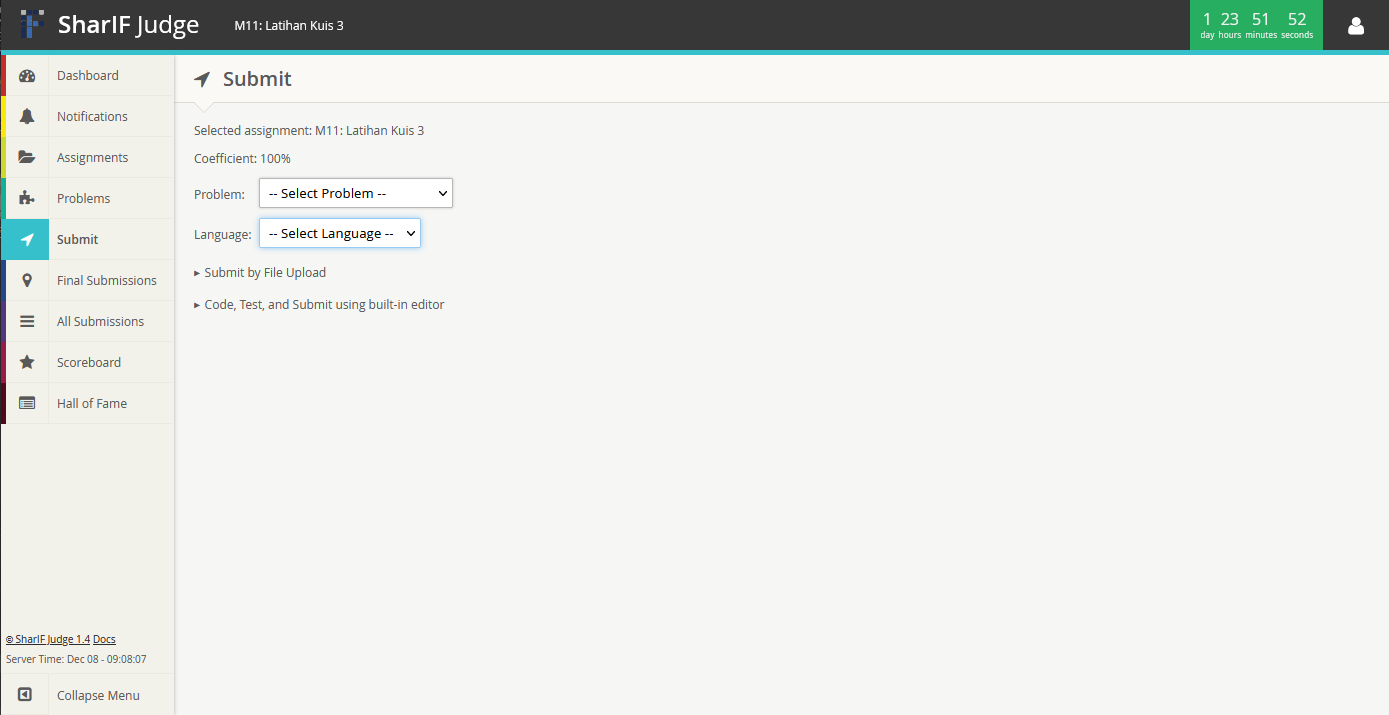
\includegraphics[scale=0.4]{Pengujian/submit_final0.PNG}  
	\caption{Tampilan antarmuka setelah perubahan}
	\label{fig:5:submit0} 
\end{figure} 

\begin{figure}[H]
	\centering  
	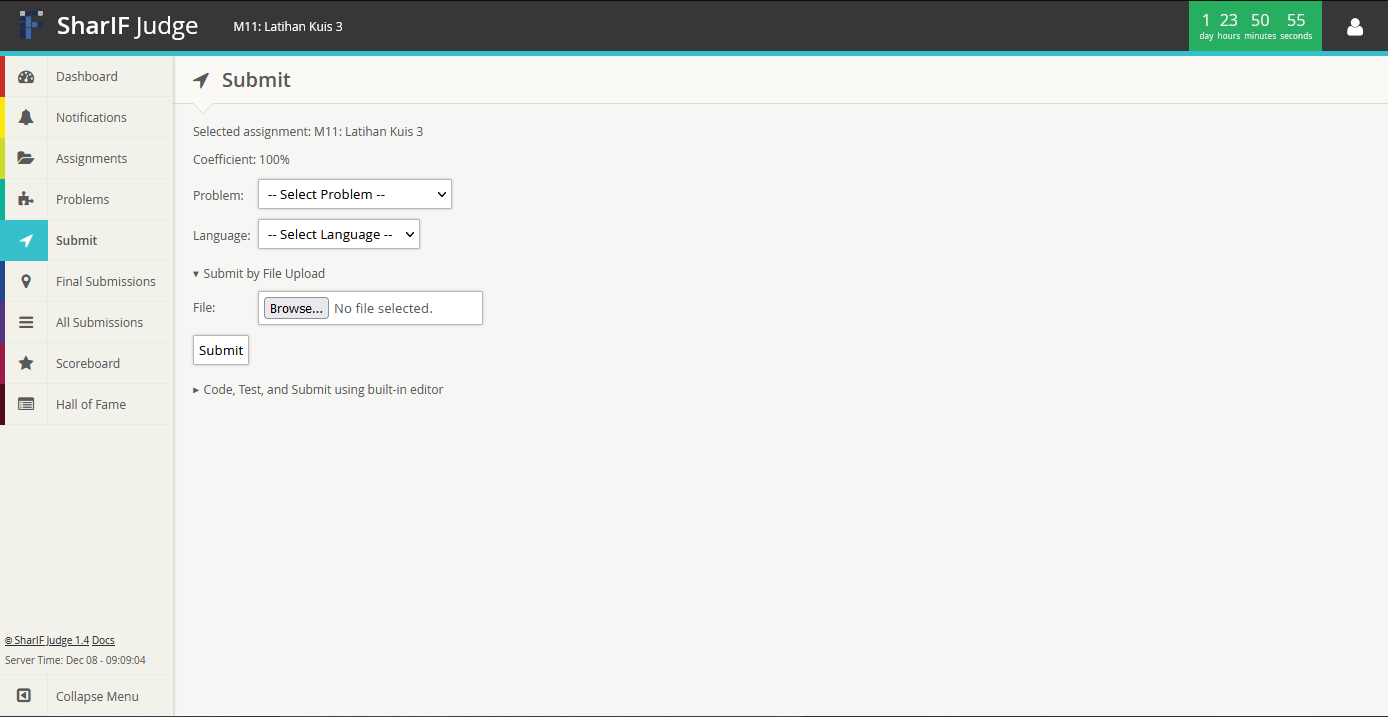
\includegraphics[scale=0.4]{Pengujian/submit_final1.PNG}  
	\caption{Tampilan antarmuka unggah \textit{file}}
	\label{fig:5:submit1} 
\end{figure} 

\begin{figure}[H]
	\centering  
	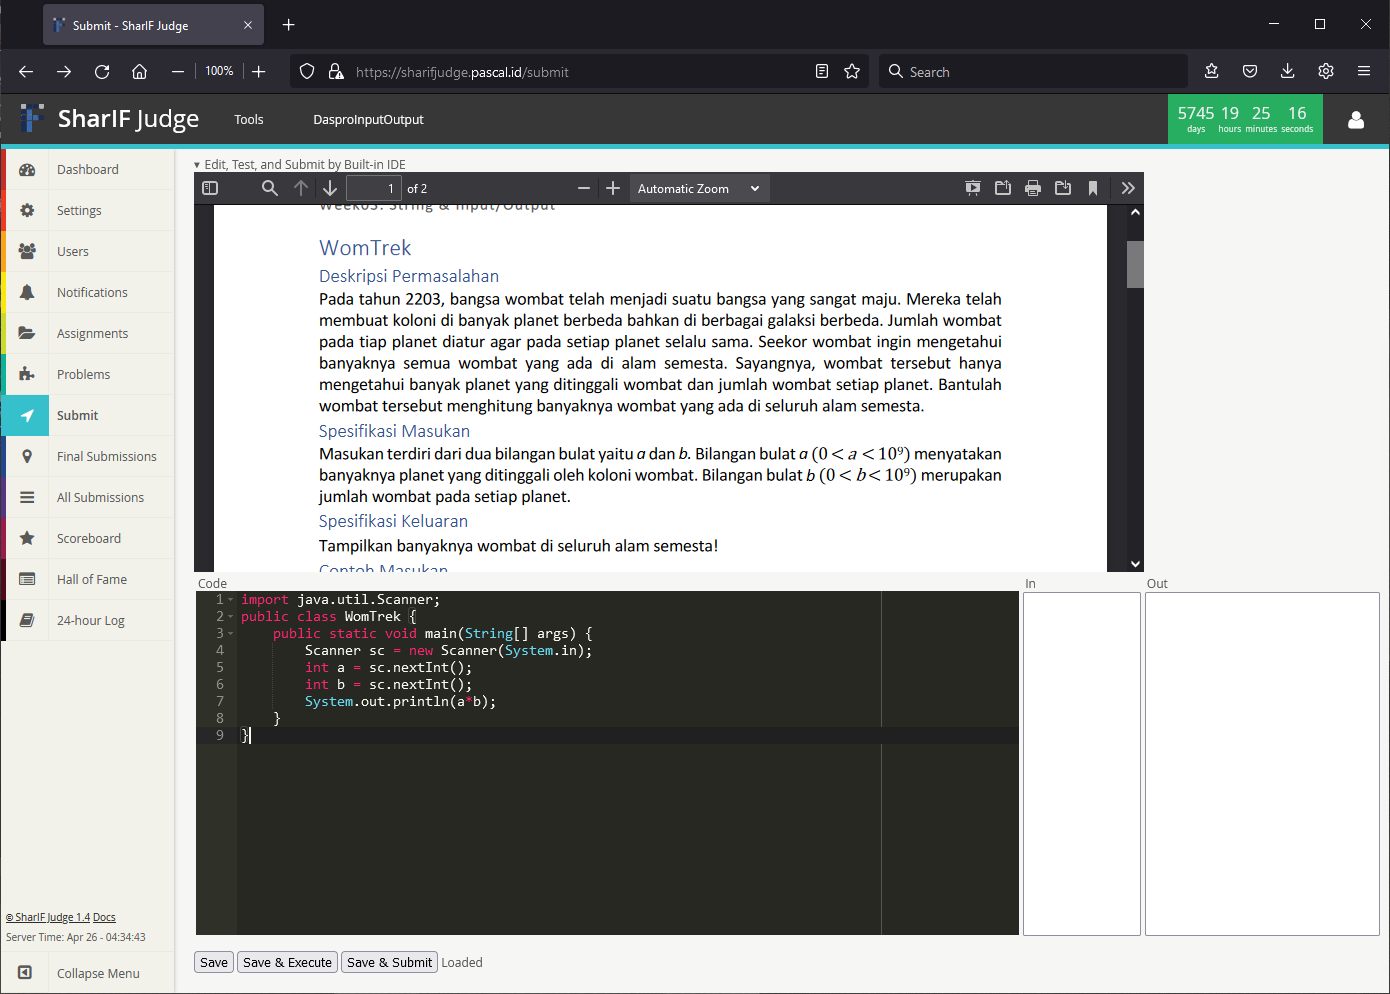
\includegraphics[scale=0.4]{Pengujian/submit_final.PNG}  
	\caption{Tampilan antarmuka IDE}
	\label{fig:5:submit2} 
\end{figure} 

Gambar \ref{fig:5:submit0} menunjukkan antarmuka halaman Submit setelah perubahan dari masukan ini. Terdapat elemen \textit{summary} pada halaman ini yang dapat ditekan untuk menampilkan antarmuka unggah file seperti pada gambar \ref{fig:5:submit1} dan antarmuka IDE seperti pada gambar \ref{fig:5:submit2}.

\subsubsection{\textit{Submit} Jawaban Soal \textit{Upload Only} Melalui IDE}
Tercatat pada \textit{issue} \#3 \footnote{https://github.com/athlonneo/SharIF-Judge/issues/3}, ditemukan masalah jika mengumpulkan jawaban untuk soal \textit{upload only}, \textit{status} pada halaman Submissions menjadi "File Not Found".

Masalah ini disebabkan karena variabel \verb|$this->problem['is_upload_only']| pada fungsi \verb|_submit| milik \textit{controller} \verb|Submit| tidak tersedia, sehingga kode dilanjutkan ke dalam antrean untuk dinilai, namun \textit{file} kunci jawaban tidak tersedia, sehingga dikembalikan \textit{status} "File Not Found".

Untuk menyelesaikan masalah ini, dimanfaatkan variabel \verb|$this->problems| yang sudah tersedia pada \textit{controller} \verb|Submit| untuk mengisi variabel \verb|$this->problem['is_upload_only']|. Perubahan ini terdapat pada kode \ref{kode:5:uosubmit} .

\begin{lstlisting}[language=diff, caption=Perubahan pada \texttt{Submit.php}, label=kode:5:uosubmit]
@@ -378,8 +378,15 @@ class Submit extends CI_Controller
                $file_fname = $file_name.'-'.($this->user->selected_assignment['total_submits']+1);
                $file_path = $user_dir.'/'.$file_fname.'.'.$file_ext;

+               foreach($this->problems as $item)
+                       if ($item['id'] == $problem_id)
+                       {
+                               $this->problem = $item;
+                               break;
+                       }
+
                if (!write_file($file_path, $data)){
                       $response = json_encode(array(status=>FALSE, message=>'Unable to submit'));
                }
\end{lstlisting}

\subsubsection{Tidak Dapat \textit{Submit} Melalui Unggah File}
Tercatat pada \textit{issue} \#7 \footnote{https://github.com/athlonneo/SharIF-Judge/issues/7}, salah satu mahasiswa mencoba melakukan \textit{submit} melalui unggah \textit{file}, namun tidak tercatat pada halaman \textit{Submissions}. Ketika mahasiswa tersebut mencoba mengunggah kode yang sama melalui IDE, \textit{submission} berhasil tercatat. 

Pada \textit{database} tabel \verb|shj_submissions|, kolom \verb|file_name| dan \verb|main_file_name| menyimpan nama \textit{file} yang diunggah. Nama \textit{file} yang diunggah ditambah dengan \verb|submit_id| untuk membedakan nama \textit{file} setiap \textit{submission}. Pada kasus ini, \verb|submit_id| sudah mencapai ratusan (3 karakter), sehingga nama \textit{file} yang diunggah mahasiswa berjumlah 31 karakter ketika ditambah dengan \verb|submit_id|. Dikarenakan kolom \verb|file_name| dan \verb|main_file_name| disimpan sebagai \verb|varchar(30)|, nama \textit{file} yang diunggah melebihi batas 30 karakter, sehingga tidak dapat disimpan pada \textit{database}.

Solusi untuk menyelesaikan masalah ini adalah dengan meningkatkan batas kolom \verb|file_name| dan \verb|main_file_name| dari menjadi \verb|varchar(100)|. Perubahan kode pada \textit{controller} \verb|Install| terdapat pada kode \ref{kode:5:dblimit}

Karena masalah ini berasal dari Sharif Judge langsung dan tidak berkaitan dengan skripsi ini, \textit{pull request} ditujukan langsung ke repositori \verb|https://github.com/ifunpar/SharIF-Judge| sebagai \textit{pull request} \#15 \footnote{https://github.com/ifunpar/SharIF-Judge/pull/15}.

\begin{lstlisting}[language=diff, caption=Perubahan pada \texttt{Install.php}, label=kode:5:dblimit]
@@ -78,8 +78,8 @@ public function index()
				'status'        => array('type' => 'VARCHAR', 'constraint' => 100),
				'pre_score'     => array('type' => 'INT', 'constraint' => 11),
				'coefficient'   => array('type' => 'VARCHAR', 'constraint' => 6),
-				'file_name'     => array('type' => 'VARCHAR', 'constraint' => 30),
-				'main_file_name'=> array('type' => 'VARCHAR', 'constraint' => 30),
+				'file_name'     => array('type' => 'VARCHAR', 'constraint' => 100),
+				'main_file_name'=> array('type' => 'VARCHAR', 'constraint' => 100),
				'file_type'     => array('type' => 'VARCHAR', 'constraint' => 6),
			);
			$this->dbforge->add_field($fields);
\end{lstlisting}

\subsubsection{\textit{Submit} Jawaban txt Melalui IDE}
Tercatat pada \textit{issue} \#10 \footnote{https://github.com/athlonneo/SharIF-Judge/issues/10}, sebelumnya IDE akan dinonaktifkan jika tipe file yang dipilih bukan bahasa program, yaitu txt dan zip. Karena editor kode dapat digunakan untuk mengedit file txt juga, disarankan untuk mengaktifkan IDE saat txt dipilih.

Perubahan dilakukan pada \verb|shj_submit.js| untuk menambahkan kondisi jika txt dipilih pada dropdown Language. Jika txt dipilih, maka editor kode akan diaktifkan dengan mode \textit{syntax highlighting} untuk \textit{plain text}. Area Input dan tombol Execute dinonaktifkan karena fitur menjalankan kode tidak dapat digunakan untuk \textit{file} txt.

\begin{lstlisting}[language=diff, caption=Perubahan pada \texttt{shj\_submit.js}, label=kode:5:uptxt]
@@ -68,6 +68,12 @@ $(document).ready(function(){
            editor.session.setMode("ace/mode/c_cpp");
            disableEditor(false);
        }
+       else if(this.value.toLowerCase().includes("txt")){
+           editor.session.setMode("ace/mode/plain_text");
+           disableEditor(false);
+           $("#editor_execute").prop("disabled", true);
+           $("#editor_input").prop("disabled", true);
+      }
        else{
            editor.session.setMode("ace/mode/plain_text");
            disableEditor(true);
\end{lstlisting}

\subsubsection{Tampilan PDF Viewer jika PDF Soal Tidak Tersedia}
Tercatat pada \textit{issue} \#11 \footnote{https://github.com/athlonneo/SharIF-Judge/issues/11}, sebelumnya PDF.js akan menampilkan pesan \textit{error} jika file PDF tidak ditemukan. Karena pesan ini kurang deskriptif bagi pengguna, disarankan untuk menyembunyikan PDF \textit{viewer} jika \textit{file} PDF soal tidak tersedia.

Pada \textit{controller} Assignments ditambahkan fungsi \verb|pdfCheck| yang mengembalikan \verb|TRUE| jika \textit{file} PDF tersedia, dan \verb|FALSE| jika \textit{file} PDF tidak tersedia. Fungsi ini akan dipanggil saat \textit{view} Submit dimuat, yang kemudian menentukan apakah PDF \textit{viewer} akan ditampilkan sesuai dengan kembalian yang didapat. Perubahan pada \textit{controller} Assignments terdapat pada kode \ref{kode:5:checkpdf}, perubahan pada \textit{view} Submit terdapat pada \ref{kode:5:viewpdf}.

\begin{lstlisting}[language=diff, caption=Perubahan pada \texttt{Assignments.php}, label=kode:5:checkpdf]
@ -588,7 +583,43 @@ class Assignments extends CI_Controller
		// redirect to add function
		$this->add();
	}
+	


+	// ------------------------------------------------------------------------
+
+
+
+	/**
+	 * Check PDF File Availability
+	 */
+	public function pdfCheck($assignment_id, $problem_id = NULL)
+	{
+		$finishtime = strtotime($this->assignment_model->assignment_info($assignment_id)['finish_time']);
+		$starttime = strtotime($this->assignment_model->assignment_info($assignment_id)['start_time']);
+		$extratime = $this->assignment_model->assignment_info($assignment_id)['extra_time'];
+
+		// Find pdf file
+		if ($problem_id === NULL || $problem_id === "null")
+			$pattern = rtrim($this->settings_model->get_setting('assignments_root'),'/')."/assignment_{$assignment_id}/*.pdf";
+		else
+			$pattern = rtrim($this->settings_model->get_setting('assignments_root'),'/')."/assignment_{$assignment_id}/p{$problem_id}/*.pdf";
+		$pdf_files = glob($pattern);
+
+		if ( ! $pdf_files )
+			$response = json_encode(array(status=>FALSE));
+		elseif (!$this->assignment_model->assignment_info($assignment_id)['open'])
+			$response = json_encode(array(status=>FALSE));
+		elseif	( ! $this->assignment_model->is_participant($this->assignment_model->assignment_info($assignment_id)['participants'],$this->user->username) )
+			$response = json_encode(array(status=>FALSE));
+		elseif ( shj_now() > $finishtime + $extratime)
+			$response = json_encode(array(status=>FALSE));
+		elseif ( shj_now() < $starttime)
+			$response = json_encode(array(status=>FALSE));
+		else
+			$response = json_encode(array(status=>TRUE));
=
+		echo $response;
+	}

}
\end{lstlisting}

\begin{lstlisting}[language=diff, caption=Perubahan pada \texttt{submit.twig}, label=kode:5:viewpdf]
@ -15,7 +15,21 @@
	<link rel="stylesheet" type='text/css' href="{{ base_url('assets/styles/submit.css') }}"/>
	<script>
		shj.p={};
-		{{ problems_js|raw }}
+		{{ problems_js|raw }};
+		$.ajax({
+            url: "{{ site_url('assignments/pdfCheck/' ~ user.selected_assignment.id) }}", 
+            cache: false,
+            success: function(data){
+				data = JSON.parse(data);
+				if(data.status){
+					$("#pdf_viewer").attr('src', "{{ base_url('assets/pdfjs/web/viewer.html?file=') ~ site_url('assignments/pdf/' ~ user.selected_assignment.id ~ '/null/true') }}");
+					$("#pdf_viewer").show();
+				}
+            },
+            error: function (error){
+                console.error(error);
+            },
+        });
	</script>
	<script src={{ base_url('assets/ace/ace.js') }}></script>
	<script type='text/javascript' src="{{ base_url("assets/js/shj_submit.js") }}"></script>
\end{lstlisting}

\subsection{Survei}
\label{subsec:survei}

Untuk mendapatkan lebih banyak masukan dari pengguna, dibuat sebuah survei untuk diisi oleh mahasiswa peserta kuliah Dasar-dasar Pemrograman. Survei ini terbagi menjadi 5 bagian untuk masing-masing fitur yang diimplementasikan pada SharIF Judge. Fitur-fitur yang terdapat pada survei adalah sebagai berikut:

\begin{enumerate}
    \item Menampilkan soal
    \item Editor kode
    \item Menyimpan dan memuat kode
    \item Menjalankan kode dengan tes kasus
    \item Mengumpulkan kode melalui IDE
\end{enumerate}

Untuk setiap fitur pada survei, terdapat 5 pertanyaan. Pertanyaan yang diberikan adalah sebagai berikut:

\begin{enumerate}
    \item Apakah Anda sudah mencoba fitur ini? (Partisipan menjawab dengan ya atau tidak)
    \item Apakah terdapat kendala saat menggunakan fitur ini? (Partisipan menjawab dengan ya atau tidak)
    \item Jika ya, apa kendala yang dialami? (Partisipan menjawab dengan kalimat sendiri)
    \item Apakah fitur ini sudah cukup nyaman untuk digunakan? (Partisipan menjawab dengan skala 1 (sangat tidak nyaman) hingga 5 (sangat nyaman))
    \item Apakah ada pendapat/saran/masukan untuk fitur ini? (Partisipan menjawab dengan kalimat sendiri)
\end{enumerate}

Pada survei ini, didapatkan respon dari 12 orang mahasiswa Dasar-dasar Pemrograman. Berikut ini adalah hasil dari survei untuk setiap fitur:

\begin{enumerate}
    \item Menampilkan soal
    \begin{enumerate}
        \begin{figure}[H]
        	\centering  
        	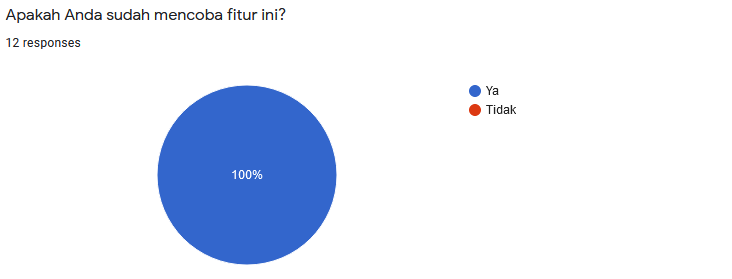
\includegraphics[scale=0.8]{Survei/11.PNG}  
        	\caption{Hasil survei bagian 1 pertanyaan 1}
        	\label{fig:5:survei11} 
        \end{figure} 
        \item Apakah Anda sudah mencoba fitur ini? \\ 100\% dari partisipan menjawab ya, hal ini menunjukkan bahwa seluruh partisipan sudah mencoba fitur ini. Hasil untuk pertanyaan ini dapat dilihat pada gambar \ref{fig:5:survei11}.
        \begin{figure}[H]
        	\centering  
        	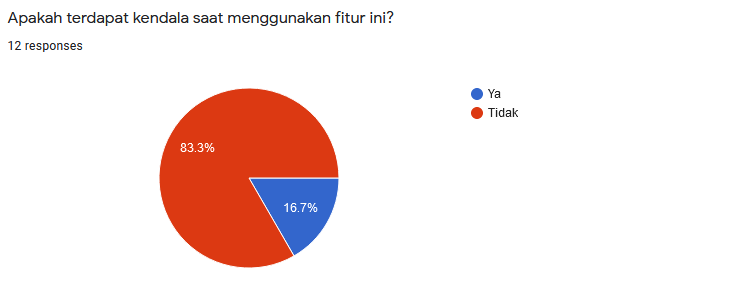
\includegraphics[scale=0.8]{Survei/12.PNG}  
        	\caption{Hasil survei bagian 1 pertanyaan 2}
        	\label{fig:5:survei12} 
        \end{figure} 
        \item Apakah terdapat kendala saat menggunakan fitur ini? \\ 83\% dari partisipan menjawab ya, hal ini menunjukkan bahwa mayoritas partisipan tidak menemukan kendala pada fitur ini. Hasil untuk pertanyaan ini dapat dilihat pada gambar \ref{fig:5:survei12}.
        \item Jika ya, apa kendala yang dialami? \\ Berikut ini kendala yang dialami:
        \begin{itemize}
            \item Pdf tidak muncul
        \end{itemize}
        \begin{figure}[H]
        	\centering  
        	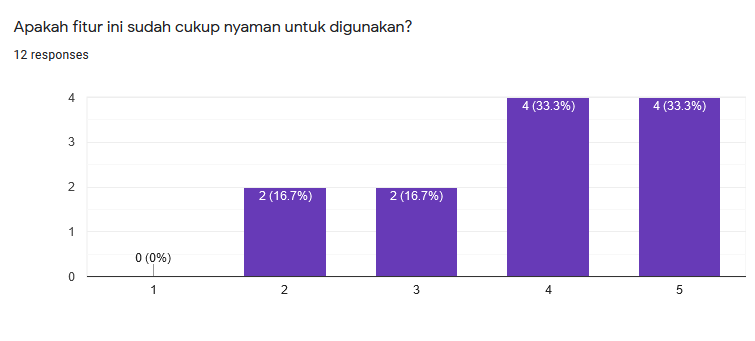
\includegraphics[scale=0.8]{Survei/14.PNG}  
        	\caption{Hasil survei bagian 1 pertanyaan 4}
        	\label{fig:5:survei14} 
        \end{figure}
        \item Apakah fitur ini sudah cukup nyaman untuk digunakan? \\ Rata-rata skor untuk pertanyaan ini adalah 3.84, dapat disimpulkan bahwa fitur ini sudah cukup nyaman untuk digunakan. Hasil untuk pertanyaan ini dapat dilihat pada gambar \ref{fig:5:survei14}.
        \item Apakah ada pendapat/saran/masukan untuk fitur ini? \\ Berikut ini adalah masukan yang didapatkan:
        \begin{itemize}
            \item Pastikan pdf bisa muncul di berbagai \textit{device}
            \item Mengubah tampilan agar soal lebih mudah dibaca
            \item Buat dark theme
        \end{itemize}
    \end{enumerate}
    \item Editor kode
    \begin{enumerate}
        \begin{figure}[H]
        	\centering  
        	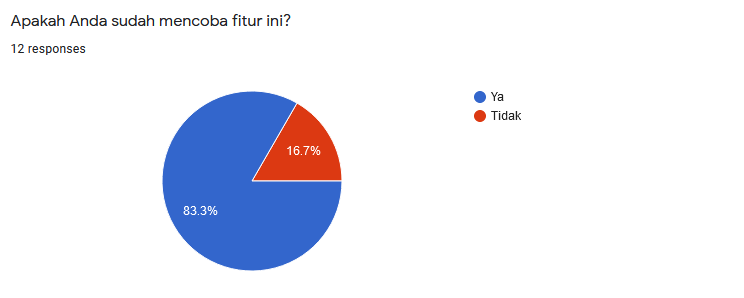
\includegraphics[scale=0.8]{Survei/21.PNG}  
        	\caption{Hasil survei bagian 2 pertanyaan 1}
        	\label{fig:5:survei21} 
        \end{figure}
        \item Apakah Anda sudah mencoba fitur ini? \\ 83\% dari partisipan menjawab ya, hal ini menunjukkan bahwa mayoritas partisipan sudah mencoba fitur ini. Hasil untuk pertanyaan ini dapat dilihat pada gambar \ref{fig:5:survei21}.
            \begin{figure}[H]
        	\centering  
        	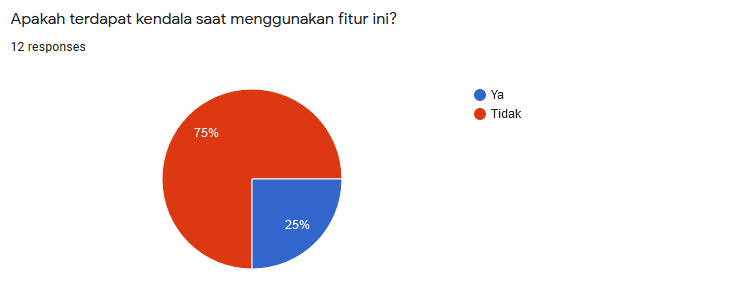
\includegraphics[scale=0.8]{Survei/22.PNG}  
        	\caption{Hasil survei bagian 2 pertanyaan 2}
        	\label{fig:5:survei22} 
        \end{figure}
        \item Apakah terdapat kendala saat menggunakan fitur ini? \\ 75\% dari partisipan menjawab tidak, hal ini menunjukkan bahwa mayoritas partisipan tidak menemukan kendala pada fitur ini. Hasil untuk pertanyaan ini dapat dilihat pada gambar \ref{fig:5:survei22}.
        \item Jika ya, apa kendala yang dialami? \\ Berikut ini kendala yang dialami:
        \begin{itemize}
            \item Terkadang jenis file tidak muncul
            \item Ukuran editor kurang besar
            \item Sulit untuk \textit{scrolling} pada text editor
        \end{itemize}
            \begin{figure}[H]
        	\centering  
        	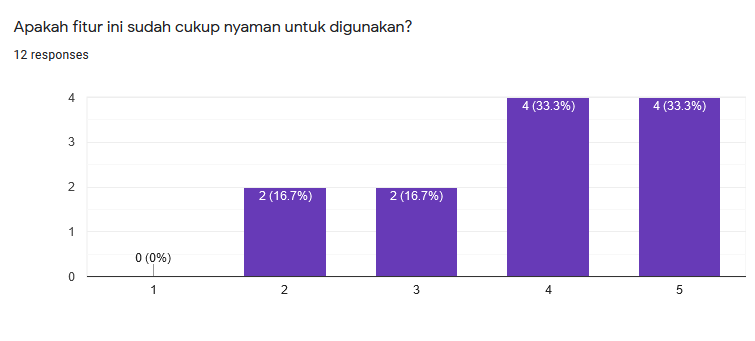
\includegraphics[scale=0.8]{Survei/14.PNG}  
        	\caption{Hasil survei bagian 2 pertanyaan 4}
        	\label{fig:5:survei24} 
        \end{figure}
        \item Apakah fitur ini sudah cukup nyaman untuk digunakan? \\ Rata-rata skor untuk pertanyaan ini adalah 4.25, dapat disimpulkan bahwa fitur ini sudah cukup nyaman untuk digunakan. Hasil untuk pertanyaan ini dapat dilihat pada gambar \ref{fig:5:survei24}.
        \item Apakah ada pendapat/saran/masukan untuk fitur ini? \\ Berikut ini adalah masukan yang didapatkan:
        \begin{itemize}
            \item Mengubah tampilan agar editor lebih mudah digunakan
        \end{itemize}
    \end{enumerate}
    \item Menyimpan dan memuat kode
    \begin{enumerate}
        \begin{figure}[H]
        	\centering  
        	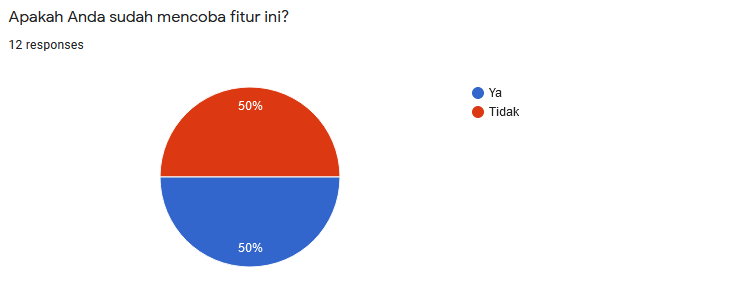
\includegraphics[scale=0.8]{Survei/31.PNG}  
        	\caption{Hasil survei bagian 3 pertanyaan 1}
        	\label{fig:5:survei31} 
        \end{figure}
        \item Apakah Anda sudah mencoba fitur ini? \\ 50\% dari partisipan menjawab ya, hal ini menunjukkan bahwa hanya sebagian partisipan sudah mencoba fitur ini. Hasil untuk pertanyaan ini dapat dilihat pada gambar \ref{fig:5:survei31}.
        \begin{figure}[H]
        	\centering  
        	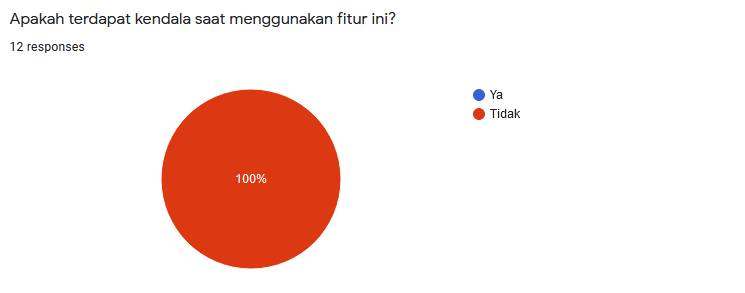
\includegraphics[scale=0.8]{Survei/32.PNG}  
        	\caption{Hasil survei bagian 3 pertanyaan 2}
        	\label{fig:5:survei32} 
        \end{figure}
        \item Apakah terdapat kendala saat menggunakan fitur ini? \\ 100\% dari partisipan menjawab tidak, hal ini menunjukkan bahwa seluruh partisipan tidak menemukan kendala pada fitur ini. Hasil untuk pertanyaan ini dapat dilihat pada gambar \ref{fig:5:survei32}.
        \item Jika ya, apa kendala yang dialami? \\ Tidak ada partisipan yang menemukan kendala pada fitur ini.
        \begin{figure}[H]
        	\centering  
        	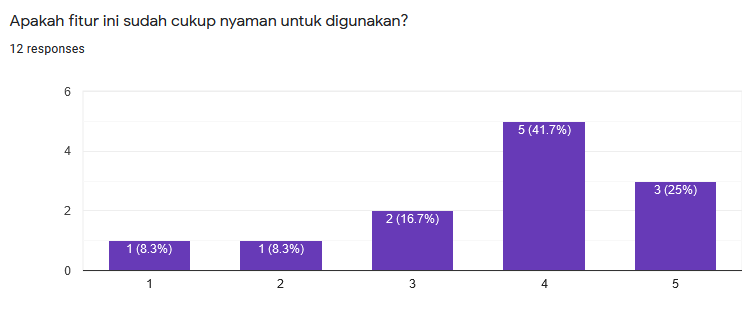
\includegraphics[scale=0.8]{Survei/34.PNG}  
        	\caption{Hasil survei bagian 3 pertanyaan 4}
        	\label{fig:5:survei34} 
        \end{figure}
        \item Apakah fitur ini sudah cukup nyaman untuk digunakan? \\ Rata-rata skor untuk pertanyaan ini adalah 3.67, dapat disimpulkan bahwa fitur ini sudah cukup nyaman untuk digunakan. Hasil untuk pertanyaan ini dapat dilihat pada gambar \ref{fig:5:survei34}.
        \item Apakah ada pendapat/saran/masukan untuk fitur ini? \\ Berikut ini adalah masukan yang didapatkan:
        \begin{itemize}
            \item Tidak perlu ada keterangan Save, cukup Execute dan Submit saja
        \end{itemize}
    \end{enumerate}
    \item Menjalankan kode dengan tes kasus
    \begin{enumerate}
        \begin{figure}[H]
        	\centering  
        	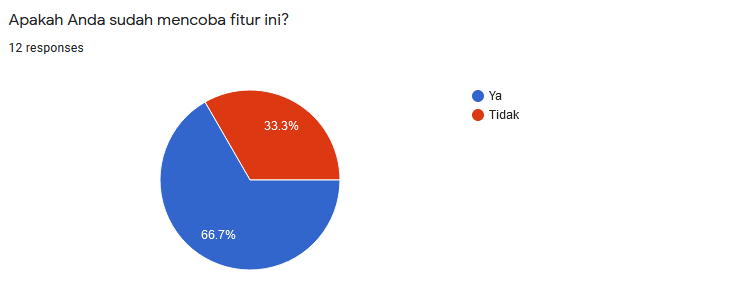
\includegraphics[scale=0.8]{Survei/41.PNG}  
        	\caption{Hasil survei bagian 4 pertanyaan 1}
        	\label{fig:5:survei41} 
        \end{figure}
        \item Apakah Anda sudah mencoba fitur ini? \\ 67\% dari partisipan menjawab ya, hal ini menunjukkan bahwa hanya sebagian partisipan sudah mencoba fitur ini. Hasil untuk pertanyaan ini dapat dilihat pada gambar \ref{fig:5:survei41}.
        \begin{figure}[H]
        	\centering  
        	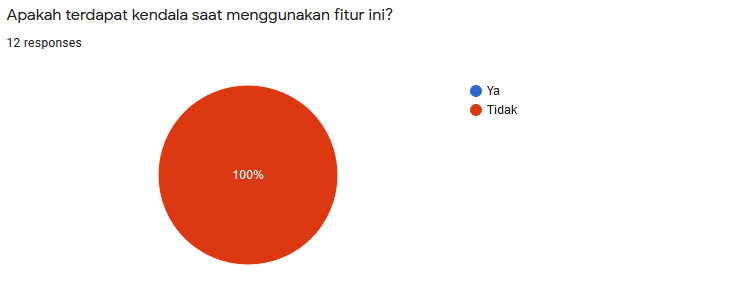
\includegraphics[scale=0.8]{Survei/42.PNG}  
        	\caption{Hasil survei bagian 4 pertanyaan 2}
        	\label{fig:5:survei42} 
        \end{figure}
        \item Apakah terdapat kendala saat menggunakan fitur ini? \\ 100\% dari partisipan menjawab tidak, hal ini menunjukkan bahwa seluruh partisipan tidak menemukan kendala pada fitur ini. Hasil untuk pertanyaan ini dapat dilihat pada gambar \ref{fig:5:survei42}.
        \item Jika ya, apa kendala yang dialami? \\ Tidak ada partisipan yang menemukan kendala pada fitur ini.
        \begin{figure}[H]
        	\centering  
        	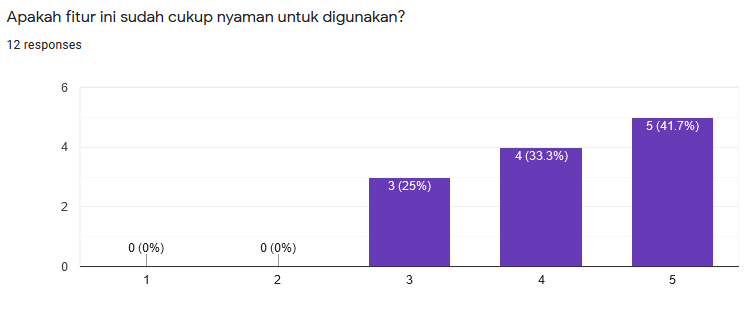
\includegraphics[scale=0.8]{Survei/44.PNG}  
        	\caption{Hasil survei bagian 4 pertanyaan 4}
        	\label{fig:5:survei44} 
        \end{figure}
        \item Apakah fitur ini sudah cukup nyaman untuk digunakan? \\ Rata-rata skor untuk pertanyaan ini adalah 4.17, dapat disimpulkan bahwa fitur ini sudah cukup nyaman untuk digunakan. Hasil untuk pertanyaan ini dapat dilihat pada gambar \ref{fig:5:survei44}.
        \item Apakah ada pendapat/saran/masukan untuk fitur ini? \\ Tidak ada partisipan yang memberi masukan pada fitur ini.
    \end{enumerate}
    \item Mengumpulkan kode melalui IDE
        \begin{enumerate}
        \begin{figure}[H]
        	\centering  
        	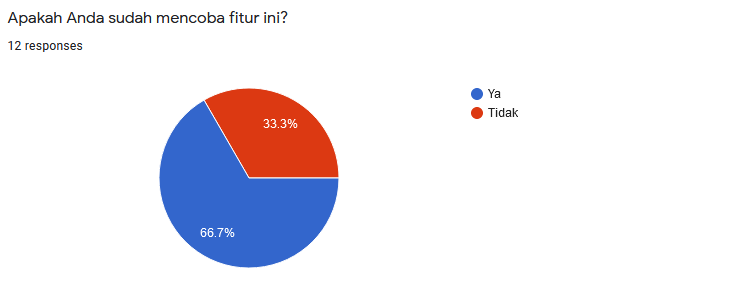
\includegraphics[scale=0.8]{Survei/51.PNG}  
        	\caption{Hasil survei bagian 5 pertanyaan 1}
        	\label{fig:5:survei51} 
        \end{figure}
        \item Apakah Anda sudah mencoba fitur ini? \\ 67\% dari partisipan menjawab ya, hal ini menunjukkan bahwa hanya sebagian partisipan sudah mencoba fitur ini. Hasil untuk pertanyaan ini dapat dilihat pada gambar \ref{fig:5:survei51}.
        \begin{figure}[H]
        	\centering  
        	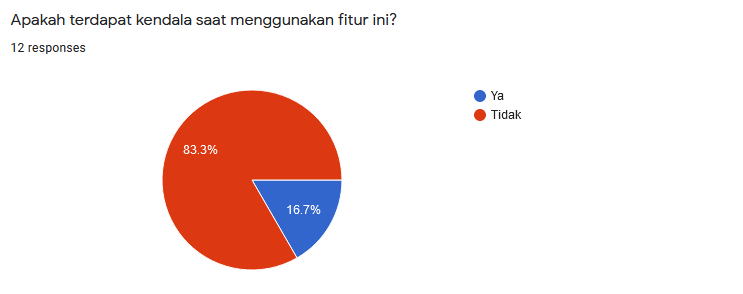
\includegraphics[scale=0.8]{Survei/52.PNG}  
        	\caption{Hasil survei bagian 5 pertanyaan 2}
        	\label{fig:5:survei52} 
        \end{figure}
        \item Apakah terdapat kendala saat menggunakan fitur ini? \\ 83\% dari partisipan menjawab tidak, hal ini menunjukkan bahwa seluruh partisipan tidak menemukan kendala pada fitur ini. Hasil untuk pertanyaan ini dapat dilihat pada gambar \ref{fig:5:survei52}.
        \item Jika ya, apa kendala yang dialami? \\ Berikut ini kendala yang dialami:
        \begin{itemize}
            \item Terkadang kode tidak terbaca di judge
        \end{itemize}
        \begin{figure}[H]
        	\centering  
        	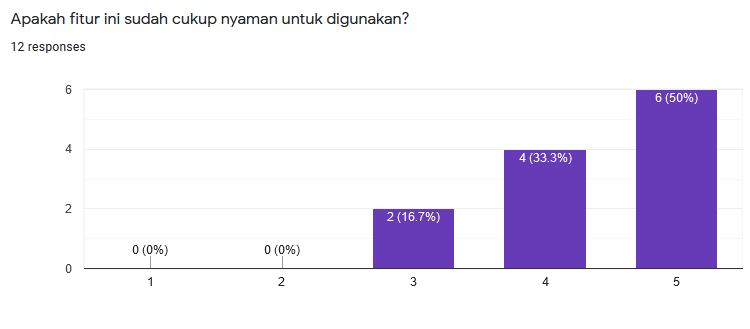
\includegraphics[scale=0.8]{Survei/54.PNG}  
        	\caption{Hasil survei bagian 5 pertanyaan 4}
        	\label{fig:5:survei54} 
        \end{figure}
        \item Apakah fitur ini sudah cukup nyaman untuk digunakan? \\ Rata-rata skor untuk pertanyaan ini adalah 4.33, dapat disimpulkan bahwa fitur ini sudah cukup nyaman untuk digunakan. Hasil untuk pertanyaan ini dapat dilihat pada gambar \ref{fig:5:survei54}.
        \item Apakah ada pendapat/saran/masukan untuk fitur ini? \\ Berikut ini adalah masukan yang didapatkan:
        \begin{itemize}
            \item Tidak perlu ada keterangan Save, cukup Submit saja
        \end{itemize}
    \end{enumerate}
\end{enumerate}

Melalui hasil survei, dapat disimpulkan bahwa fitur-fitur yang diimplementasikan pada SharIF Judge sudah cukup nyaman untuk digunakan. Sebagian besar masukan dan kendala pada umumnya berkaitan dengan antarmuka. Masih banyak mahasiswa yang belum mencoba fitur menyimpan, menjalankan, dan mengumpulkan kode. Hal ini kemungkinan disebabkan karena mahasiswa didorong untuk menggunakan IDE BlueJ selama kelas Dasar-dasar Pemrograman, yang menyebabkan mahasiswa tidak mencoba untuk menggunakan fitur IDE pada SharIF Judge.